\chapter{Background Material}
\label{chap:chap2}
\newcommand*{\PathChapter}{../Chapter2}%

This chapter aims to set the context for the remainder of this thesis. Various concepts pertaining to this thesis, including Bayesian inference, exponential family distributions and differential privacy, are briefly introduced in the following.

\section{Comparing probability distributions}
\label{subsec:b-divergences}
Throughout the thesis we focus primarily on probability spaces equipped with measures that are absolutely continuous~\wrt~some base measure, corresponding to the Lebesgue and counting measure respectively when considering continuous and discrete mappings from the sample space. This allows us to simplify notation and adapt the definitions presented in this section to normalised probability densities.
 
A critical component in constructing and evaluating inference algorithms is using a \emph{divergence measure}, that captures informatively how similar two probability distributions are. Statistical divergences are relaxations of distance functions, that (\emph{i})~are always non-negative, and (\emph{ii})~equal zero iff their arguments are identical---albeit they do not necessarily satisfy symmetry in their arguments, or the triangle inequality, hence not having to be a metric by virtue of definition. 

The most commonly used divergence measure in approximate inference---which will directly serve to define the objective quantifying the inferential quality of our sparse approximations in~\cref{chap:chap4,chap:chap5}---is the \emph{Kullback-Leibler}~(KL) divergence, also named \emph{relative entropy}~\citep{kullback51,kullback59}. For a continuous random variable $\theta$ and probability density functions $\pi_1$ and $\pi_2$, the KL divergence is defined as 
\[
\label{eq:bkl-def}
\kl{\pi_1}{\pi_2} \defined \int \pi_1(\theta) \log\frac{\pi_1(\theta)}{\pi_2(\theta)} d\theta.
\]
In particular, for two $d$-dimensional Gaussian distributions $\mcN_1(\mu_1, \Sigma_1)$ and $\mcN_2(\mu_2, \Sigma_2)$, the KL divergence is computable in closed form as follows
\[
\kl{\pi_1}{\pi_2} = \frac{1}{2}\left[\log\frac{|\Sigma_2|}{|\Sigma_1|} - d  + \tr(\Sigma_2^{-1}\Sigma_1) + (\mu_2-\mu_1)^T\Sigma_2^{-1}(\mu_2-\mu_1) \right].
\]

%\section{Robust Inference}
%\label{sec:b-robust-inference}
In data setups that are likely to be contaminated by outliers, we get substantial inferential performance improvements when enhancing our algorithms with statistical~\emph{robustness}. Relying on the KL divergence cannot sufficiently address this concern, as this divergence attaches great importance to correctly capturing the tail behaviour of the observations. A robustified divergence, termed~\emph{\bdiv{}} or \emph{density power divergence}, was instead proposed in~\citep{basu98,eguchi01}, that is able to downweight outlying datapoints. Considering again the densities $\pi_1, \pi_2$, the \bdiv{} is defined as 
\[
\betadistance{\pi_1}{\pi_2} \defined \frac{1}{\beta(\beta+1)} \displaystyle \int \left( \pi_1(\theta)^{1+\beta} - (\beta+1) \pi_1(\theta) \pi_2(\theta)^{\beta}  +  \beta \pi_2(\theta)^{1+\beta} \right)d\theta,
\] 
for $\beta \in \reals\setminus\{-1, 0\}$.

One can easily show that the \bdiv{} converges to the KL divergence when $\beta \rightarrow 0$.
Both divergences are asymmetric and do not satisfy the triangle inequality. Moreover, both divergences are instances of the family of Bregman divergences~\citep{amari16,banerjee05,cichocki10}, \ie{} a class of dissimilarity measures that can be expressed as $d_\phi(p, q) = \phi(p) - \phi(q) - \langle \grad\phi(q), p-q \rangle$ using a strictly convex, differentiable function $\phi: \mcK \rightarrow \reals$, for all $p, q$ in a convex set $\mcK \subseteq	\reals^d$. In the case of two probability density functions $\pi_1, \pi_2$ the Bregman divergence admits the form $D_\phi(\pi_1, \pi_2) = \displaystyle\int \left[\phi(\pi_1(\theta)) - \phi(\pi_2(\theta)) - \phi'(\pi_2(\theta))(\pi_1(\theta)-\pi_2(\theta))\right]d\theta$. The convex functions defining the corresponding divergences are presented in~\cref{table:bregman-reductions}.

\begin{table}[!t]
	\begin{center}
		\begin{tabular}{|l|l|l|}
			\hline
			\textsc{Divergence}     & $\phi(\xi)$     \\ \hline
			\text{Kullback-Leibler} & $ \xi \log\xi $   \\ \hline 
			\text{\bdiv{}}  & $\frac{1}{\beta(\beta+1)}\xi^{\beta+1} - \frac{1}{\beta} \xi + \frac{1}{\beta+1}, \;\; \beta > 0$  \\ \hline
		\end{tabular}
	\end{center}
	\caption{Convex functions used for reductions of relative entropy and density power to Bregman divergences on the domain of probability density functions.}
	\label{table:bregman-reductions}
\end{table}


\section{Exponential families}
\label{sec:b-expfam}

The exponential family~\citep{wainwright08} is a broad class of probability distributions, sharing a set of important properties that facilitate tractable inference. Exponential family members include numerous well-known distributions, such as the Poisson distribution, the Gamma distribution, and the Gaussian or normal distribution. 

\begin{ndefn}[Exponential family] \label{def:bexpfam}
	A collection of densities $\pi$, with respect to a base measure $\nu$ indexed by a vector of parameters $\theta$, is an \emph{exponential family} of densities if it can be written as
	\[
	\pi_{\theta}(x) = h(x) \exp\left( \langle \theta, t(x) \rangle - Z(\theta) \right).
	\label{eq:bexpfam}
	\]
	We call $t(x): \mcX \rightarrow \reals^{d}$ the \emph{sufficient statistics} of the data, $h(x)$ the \emph{base density} and 
	\[
	Z(\theta)\defined \log \int e^{\langle \theta, t(x) \rangle } h(x) \nu(dx)
	\label{eq:b-logpartition}
	\]
	the \emph{log-partition function}.
\end{ndefn}

The parameter space of interest, referred to as the \emph{natural parameter space}, is the space $\Omega \subseteq \reals^d $ that contains all $\theta$ such that $Z(\theta)$ is finite. We say that a family is \emph{regular} if $\Omega$ is open.

An important property of exponential family densities is that the derivatives of the log-partition function $Z$ are related to the moments of the sufficient statistics as follows.

\begin{nprop}[Derivatives of the log-partition function via expected statistics] \label{prop:bgradZ}
	For a regular exponential family of densities in the form of~\cref{eq:bexpfam}, the log-partition function has derivatives of all orders on its domain $\Omega$, while for the first two derivatives hold the following
	\[
	\grad Z(\theta) = \EE_{\theta}[t(x)]
	\label{eq:bgradZ}
	\] 	
	and 
	\[
	\grad^2Z(\theta) = \cov_{\theta}[t(x)] \defined \EE_{\theta}[t(x)t(x)^T] - \EE_{\theta}[t(x)]\EE_{\theta}[t(x)]^T.
	\label{eq:bhessZ}
	\]
\end{nprop}

\cref{prop:bgradZ} allows efficient approximations for the gradient and Hessian of $ Z $ using empirical estimates of the first two moments of the sufficient statistic; we take advantage of this property in the variational inference schemes to be introduced in~\cref{chap:chap4,chap:chap5}.

\section{Probabilistic learning at  a glance}
\label{sec:b-bayesian-inference}

Bayesian probabilistic modeling provides a principled framework for  learning from observed data, incorporating expert knowledge, handling model uncertainty and drawing coherent inferences in a unified way, following the languange of probability theory.

In (parametric) Bayesian learning settings we are generally given a set of observations $x = \{x_1,...,x_N\} \subseteq \mcX$, and aim to find a vector of random variables $\theta $ parameterising an assumed probabilistic model that \emph{is likely to} explain them. In the Bayesian paradigm, we first assume a \emph{prior} distribution over the parameters $\pi_0(\theta)$, that encodes our beliefs about the uncertainty in $\theta$ before observing any data. Once the data are taken into account, our beliefs shoud be updated accordingly, in order to better describe the observed distribution. For this purpose a \emph{likelihood} function $\pi(x|\theta)$ needs to be defined; the likelihood quantifies the probability of the observations under the assumed statistical model for parameters set to $\theta$. Combining the above distributions we are ready to formulate \emph{Bayes' theorem}, the fundamental rule which gives the \emph{posterior} beliefs for our parameters updated in light of the observed data
\[
\pi(\theta|x) = \frac{\pi(x|\theta)\pi_0(\theta)}{\pi(x)}.
\label{eq:bbayes-rule}
\] 
Henceforth any quantity of interest $g(\cdot)$ involving the assumed probabilistic model is calculated using expectations under the posterior---which is considered to be the complete information about $\theta$ given the data $x$---as follows
\[
\EE_{\theta \sim \pi(\theta|x)}\left[g(\theta)\right] \defined \int g(\theta) \pi(\theta|x) d\theta.
\label{eq:binference}
\]
Computing~\cref{eq:binference} is known as doing \emph{inference} on our statistical model.

A key challenge in computing the posterior according to~\cref{eq:bbayes-rule} is evaluating the normalizer, called \emph{marginal likelihood} (or \emph{model evidence}), which in a continuous parametric space takes the form
\[
\pi(x) = \int \pi(x|\theta) \pi_0(\theta) d\theta.
\label{eq:bmarginal-likelihood}
\]
\emph{Marginalising}, \ie~computing the integral of~\cref{eq:bmarginal-likelihood}, can be done using analytical tools for a number of simple Bayesian models---some of which will be discussed in the remainder, including Gaussian mean inference, Bayesian and neural linear regression---where the likelihood is conjugate to the prior. However, for the vast majority of interesting statistical models marginalization cannot be done in closed form and should be approximated instead. Aiming to address such cases, approximate Bayesian inference has emerged as an active research area for many decades. In the remainder of the section we present an overview of existing approaches addressing approximate inference that are relevant to our algorithms. For a more detailed exposure, including methods beyond the scope of this thesis (e.g. expectation propagation), cf.~\citep{bishop06,murphy12,angelino16}.

\subsection{Laplace's method}
\label{subsec:b-laplace-method}

Point estimates of $\theta$, obtained for example via \emph{maximum a posteriori} or \emph{maximum likelihood estimation}, are cheap to compute, as they correspond to solutions of optimization problems involving only the unnormalised RHS of~\cref{eq:bbayes-rule}---on the other hand, they cannot capture the uncertainty of our posterior beliefs. Laplace's method~\citep{mackay03} is an approximate inference scheme that makes a first step towards uncertainty awareness, offering a non-degenerate, yet inexpensive to compute, approximate posterior for $\theta$.

Let us write the posterior of~\cref{eq:bbayes-rule} in the following equivalent form
\[
\pi(\theta|x) = \frac{1}{Z} e^{-E(\theta)},
\]
where $E(\theta) \defined - \log \pi(\theta, x)$ is called the \emph{energy function}, and $ Z $ is the unknown normalization constant. Taking the Taylor series expansion of $\theta$ (up to order 2) around the mode $ {\htheta \defined \arg \underset{\theta}{\min} \;E(\theta)}$, we obtain the approximation 
$ \hpi(\theta, x) := e^{-E(\htheta)}\exp\left((\theta - \htheta)^T\Lambda (\theta - \htheta)\right)$ where  $ \Lambda \defined -\grad^2 E(\theta)\Big|_{\theta = \htheta}$.
Hence we have
\[
\pi(\theta|X) \approx \frac{1}{Z}   \hpi(\theta, x)  \propto \mcN(\htheta, \Lambda^{-1}), 
\label{eq:blaplace-approx}
\]  
\ie~the posterior can be approximated by a (unimodal) Gaussian, where the mean corresponds to the minimum of the energy function and the covariance is the negative Hessian of the energy function evaluated on the mean. Clearly, using standard numerical optimization routines, e.g. quasi-Newton methods, we can achieve fast convergence to $\htheta$. 

Laplace approximations will be used as coarse posterior approximations over our coreset summary constructions.

\subsection{Sampling methods}
\label{subsec:b-sampling-methods}
In the absence of analytical formulae, integrals in the form of~\cref{eq:binference} can be approximated via empirical averaging, using samples from the target posterior distribution
\[
 \int g(\theta) \pi(\theta|x) d\theta \approx \frac{1}{S} \sum_{s=1}^{S} g(\theta_s), \quad (\theta_s)_{s=1}^{S} \distiid \pi(\theta|x) .
\]
\emph{Markov Chain Monte Carlo~(MCMC)}, the workhorse of approximate Bayesian inference, is a framework of established tools that pursue the above idea efficiently~\citep{geyer92, gilks05, robert05}. 

MCMC offers approximations to expectations \wrt intractable probability distributions via simulating an ergodic random walk in the state space of the model, which admits the true posterior as its stationary distribution. As implied by the strong law of large numbers, the MC estimate---formed using (effectively independent) samples from the stationary distribution---converges to the true expectation almost surely as $s \rightarrow \infty$; this property makes MCMC methods theoretically appealing, as it endows the estimators with strong \emph{asymptotic exactness} guarantees. Moreover, if $g$ is a real function, using the central limit theorem, it can be shown that the standard error of a MC estimator scales asymptotically as $O(\frac{1}{\sqrt{S}})$, independently of the dimension of $\theta$. Differing in the way that the Monte Carlo chain is constructed, as well as the offered level of automation, several methods of MCMC inference have emerged, including the Metropolis-Hastings~\citep{andrieu03}, the Hamiltonian Monte-Carlo~\citep{neal11}, and the No-U-Turn-Sampler~(NUTS)~\citep{hoffman14}. NUTS will be used as a reference method to evaluate summarization performance in part of our experiments over~\cref{chap:chap4,chap:chap5}.

The computation of bounds on the number of MCMC iterations required until we obtain a satisfactory posterior approximation can hardly be automated, as they are highly problem-specific, and in practice heuristics are used to decide when sampling should stop. Typically each sample requires at least one evaluation of a function proportial to $\pi$, scaling at cost $\Theta(N)$ which becomes a burden in big data applications---on this account, methods operating on data subsets have been proposed, including~\citep{welling11,korattikara14,bardenet14}. Despite these shortcomings, in settings where data are high-dimensional, and likelihood surface lacks structure that could be exploited over inference, MCMC remains the gold standard for practitioners.



\subsection{Variational inference}
\label{subsec:b-variational-inference}
Variational inference~(VI)~\citep{jordan99,blei17} takes a fundamentally different approach to addressing approximate inference.
The problem formulation underpinning all VI methods is to find a member $q^*$ within a family of tractable probability densities $Q$ that most closely matches our true posterior $\pi$ (typically in the KL-sense)
\[
\label{eq:bvi}
q^{*}(\theta; x) \defined \arg \underset{q\in Q}{\min} \kl{q(\theta)}{\pi(\theta|x)}.
\]
In this way, Bayesian posterior inference gets reduced into an optimization problem; hence, techniques allowing scaling up optimization (e.g. random subsampling) can in principle be applied in VI methods, enabling scalable inference of approximate posteriors~\citep{hoffman13}.

We note in passing that, in classical Variational Bayes schemes, expanding the KL divergence according to~\cref{eq:bkl-def} makes the log-evidence appear in the objective 
\[
\kl{q(\theta)}{\pi(\theta|x)} = \EE_{\theta \sim q}\left[\log q(\theta)\right] - \EE_{\theta \sim q}\left[\log \pi(x, \theta)\right] + \log \pi(x).
\]
Since this term is not a function of $q$, it can be subtracted and the problem is reformulated as minimizing the remaining two terms, the negation of which is known as the \emph{evidence lower bound}~(ELBO)
\[
q^{*}(\theta; x) \defined \arg \underset{q\in Q}{\min} \left(-\text{ELBO}(q, x)\right), \qquad
\text{ELBO}(q, x) \defined \EE_{q}\left[\log \pi(x, \theta)\right] - \EE_q \left[\log q(\theta)\right].
\]
Via Jensen's inequality, the ELBO can be shown to be a lower bound of the marginal log-likelihood of $x$ as expectation \wrt~$q$. As opposed to MCMC methods, theoretical guarantees for inferential results of the solution to~\cref{eq:bvi} can only be obtained for a few simple statistical models for the following main reasons: optimization methods in typically non-convex landscapes can often converge to bad local optima; also, depending on the statistical divergence and variational family used, VI might return miscalibrated posterior variance estimates~\citep[Chapter~10]{bishop06}.

The simplest family $Q$ that can be used for VI is the \emph{mean-field variational family} which relies on the simplifying assumption of independence among the coordinates of $\theta$, \ie~$q(\theta) \defined \Pi_{d=1}^{D}q_d(\theta_d)$.
Our VI schemes in~\cref{chap:chap4,chap:chap5} propose approximations within the \emph{exponential family} instead, which generally allow less restricted posteriors. Additionally, they can circumvent the use of ELBO, and instead be directly applied on the original KL minimizing variational formulation of~\cref{eq:bvi}, since MC estimates of the gradient of the intractable log-evidence term can be extracted as per~\cref{prop:bgradZ}. 

\subsection{Bayesian coresets}
\label{subsec:b-coresets}
Owing to their requirement for multiple evaluations of the data (log-)likelihood---a computation scaling at $\Theta(N)$---MCMC and VI methods quickly become prohibitively expensive in the large-data regime. Various stochastic schemes have been proposed to circumvent this computation, evaluating the likelihood on random data minibatches: despite achieving computational savings and often being straightforward to implement, such schemes rarely offer guarantees on posterior approximation quality, and lack a rigorous principle over the minibatch selection step, hence retaining part of the redundancy of the full data collection in the extracted samples.

Bayesian coresets~\citep{huggins16,campbell18,campbell19jmlr,campbell19neurips,zhang21} make the assumption that the full dataset has some degree of inherent redundancy, and put forth the idea of scaling up inference via the application of a preprocessing step where \emph{part of the data gets retained under the criterion of likelihood approximation}. In the spirit of the first coresets proposed in the field of computational geometry~\citep{feldman11unified}, initial construction schemes for coreset-based \mbox{inference~\citep{huggins16,lucic17training}} utilize \emph{importance sampling} according to the datapoints' sensitivity, \ie~a non-negative quantity measuring the redundancy of each of the datapoints \wrt the statistical model of interest. Although providing theoretical guarantees for the approximation quality achieved by the coreset, importance sampling based constructions have typically two shortcomings: (\emph{i}) they rely on efficiently computable upper bounds of the sensitivity, and (\emph{ii}) they do not have a sense of a residual posterior error, hence are limited by common MC rates in approximating the full data likelihood, offering error $\eps = O(\frac{1}{\sqrt{M}})$ for coreset size $M$.

Reformulating coreset construction as sparse function approximation in a Hilbert space~(\emph{Hilbert coresets}),~\textcitec{campbell18,campbell19jmlr} introduced alternative optimization formulations for the problem. They showed that using inner-product inducing norms can lead to faster incremental construction schemes that, critically, can guide next datapoint selection by the direction of greatest impovement. Moreover, they made use of a coarse posterior approximation and random projections to efficiently compute Hilbert norms that capture the divergence between the coreset and the true posterior, and proposed faster sparse constructions under polytope and hypersphere constraints.

In more recent work,~\textcitecustom{campbell19neurips} casted Bayesian coresets to a problem of sparse variational inference within an exponential family, named \emph{Riemannian coresets}. Riemannian coresets removed the requirement for fixing a coarse posterior that appears when computing the norm in practical Hilbert coreset constructions, achieving full automation and improvement of approximation quality (measured through the KL divergence) over a larger range of summary sizes.


\section{Robust inference}
\label{sec:brobust-inference}

In this section, adopting an optimization perspective of Bayesian inference, we present robustness limitations of the standard Bayesian posterior on big data, and outline existing generalizations of the posterior that aim to robustify inference \wrt mismatches between observed data and modelling assumptions. Setting these robustified posteriors as the target of our coreset approximations, in~\cref{chap:chap5} we will successfully address scenarios of large-scale inference under model misspecification.

\subsection{Standard Bayesian inference and lack of robustness in the large-data regime}
In the context of Bayesian inference, we are interested in updating our beliefs about a vector of random variables $\theta \in \Theta$, initially expressed through a prior distribution $\pi_0(\theta)$, after observing a set of datapoints $ x:=(x_n)_{n=1}^{N} \in \mcX^N$. Here we equivalently rewrite~\cref{eq:bbayes-rule} as
\[
\pi(\theta|x) = \frac{1}{Z'}\pi(x|\theta)\pi_0(\theta),
\label{eq:bayes-rule}
\] 
where $Z'$ is a normalization constant corresponding to the (typically intractable) marginal likelihood term $\pi(x)$. %, and $\pi(x|\theta)$ is the likelihood of our observations according to an assumed statistical model.
When the datapoints $x$ are conditionally independent given $\theta$, the likelihood function gets factorized as \mbox{$\pi(x|\theta) = \Pi_{n=1}^{N}\pi(x_n|\theta)$.} An equivalent formulation of  the
Bayesian posterior as a solution to a convex optimization problem over the density space was introduced by~\textcitec{williams80} and~\textcitec{zellner88}, and used in various subsequent works including~\citep{zhu14, dai16, futami18}. Concretely,~\cref{eq:bayes-rule} can be recovered by solving the problem
\[
\arg \underset{q(\theta) \in \mcP}{\min} \left(\kl{q(\theta)}{\pi_0(\theta)} -\sum_{n=1}^{N}\left[\int q(\theta) \log \pi(x_n|\theta)d\theta\right]\right),
\label{eq:bayes-rule-opt}
\]
where $\mcP$ is the valid density space, while the Bayesian posterior can be expressed as 
\[
\pi(\theta|x) = \frac{1}{Z'} \exp\left(-\xent{\hpi(x)}{\pi(x|\theta)}\right)\pi_0(\theta).
\label{eq:zellner-rule}
\]
In the last expression, $\hpi(x):=\frac{1}{N}\sum_{n=1}^{N}\delta(x-x_n)$ is the empirical distribution of the observed datapoints and $\delta$ is the Dirac delta function. The exponent $\xent{\hpi(x)}{\pi(x|\theta)}:=-\sum_{n=1}^{N}\log\pi(x_n|\theta)$
corresponds (up to a constant) to the \emph{cross-entropy}, which is  equal to the empirical average of negative log-likelihoods of the datapoints, and quantifies the expected loss incurred by our estimates for the model parameters $\theta$ over the available observations, under the Kullback-Leibler divergence.

When $N$ is large, the Bayesian posterior is strongly affected by perturbations in the observed data space. To develop an intuition on this, assuming that the true and observed data distributions admit densities $\pi_\theta$ and $\pi_\textsubscript{obs}$ respectively, we can rewrite an approximation of~\cref{eq:zellner-rule} via the KL divergence as in~\citep{miller19}
\[
\pi(\theta|x) 
& \propto  \exp\left(\sum_{n=1}^{N}\log\pi(x_n|\theta)\right) \pi_0(\theta)
\doteq	 \exp\left(N \int \pi_\textsubscript{obs} \log \pi_\theta\right) \pi_0(\theta) \notag \\
&:= \exp\left(-N \kl{\pi_\textsubscript{obs}}{\pi_\theta}\right) \pi_0(\theta),
\label{eq:missmatch_with_N}
\]
where $\doteq$ denotes  agreement to first order in exponent.\footnote{\ie~$a_n \doteq b_n$ iff $(1/n)\log(a_n/b_n) \rightarrow 0$}
Hence, due to the large $N$ in the exponent, small changes in $\pi_\textsubscript{obs}$ will have a large impact on the posterior.

\subsection{Robustified generalized Bayesian posteriors}

Robust inference methods aim to adapt~\cref{eq:bayes-rule,eq:bayes-rule-opt,eq:zellner-rule} to formulations that can address the case of observations departing from model assumptions, as often happening in practice, e.g. due to misspecified shapes of data distributions and number of components, or due to the presence of outliers. In such formulations~\citep{dawid16, jewson18, fujisawa08, eguchi01}, Bayesian updates rely on utilising robust divergences instead of the KL divergence, to express the losses over the observed data. 

From the definition of KL divergence~\cref{eq:bkl-def}, we can equivalently rewrite \cref{eq:bayes-rule-opt} as
\[
\arg \underset{q(\theta) \in \mcP}{\min}  \left(\kl{q(\theta)}{\pi_0(\theta)} + N\EE_{q(\theta)}\left[\kl{\hpi(x)}{\pi(x|\theta)}\right]\right),
\label{eq:bayes-rule-opt-kl}
\]
namely inference corresponds to maximizing the expected likelihood of the observations, under a regularizer that aims to keep the posterior $q$ close to the prior $\pi_0$.
As mentioned in~\cref{subsec:b-divergences}, a popular choice for enhancing inferential robustness is to replace the KL divergence---computed via the expected likelihood  arising in the second term of~\cref{eq:bayes-rule-opt-kl}---with the \emph{\bdiv}~\citep{futami18, knoblauch18}. This yields the following posterior for $\theta$~\citep{ghosh16,knoblauch18}
\[
\pi_\beta(\theta|x) \propto \exp\left(-\db{\hpi(x)}{\pi(x|\theta)}\right)\pi_0(\theta),
\label{eq:b-posterior}
\] 
where 
\[
\db{\hpi(x)}{\pi(x|\theta)} := 
\sum_{n=1}^{N}  \underbrace{\left(-\frac{\beta+1}{\beta}\pi(x_n|\theta)^{\beta} + \int_{\mcX} \pi(\chi|\theta)^{1+\beta}d\chi\right)}_{:=f_n(\theta)},
\label{eq:b-loss}
\]
with $\beta>0$.
In the remainder of the thesis we refer to quantities defined in~\cref{eq:b-posterior,eq:b-loss} as the \emph{\bpost{}} and \emph{\blik{}} respectively. Noticeably, the individual terms $f_n(\theta)$  of the \blik{} allow attributing \emph{different strength of influence to each of the datapoints}, depending on their accordance with the model assumptions. As densities get raised to a suitable power $\beta$, outlying observations are exponentially downweighted. When $\beta \rightarrow 0$, the Bayes' posterior of \cref{eq:bayes-rule,eq:zellner-rule} is recovered, and all datapoints are treated equally.

In the presentation above we focused on modeling observations $(x_n)_{n=1}^{N}$~(unsupervised learning). In the case of supervised learning on data pairs ${(x_n,y_n)}_{n=1}^{N} \in (\mcX \times \mcY)^N$, the respective expression for individual terms of the \blik{}\footnote{In this context for simplicity we use notation $f_n(\cdot)$  to denote $f(y_n|x_n, \cdot)$.} is~\citep{basu98}
\[
f_n(\theta):= -\frac{\beta+1}{\beta}\pi(y_n|x_n,\theta)^{\beta} +  \int_{\mcY} \pi(\psi|x_n,\theta)^{1+\beta}d\psi.
\label{eq:sl-lik-terms}
\] 

\textbf{Illustrations}~~
In the remainder of this section we illustrate the effects of adapting the used statistical divergence when doing inference on a dataset that contains outliers. In a similar vein to~\citep{jewson18}, we juxtapose the inference results of classical and robust posterior on simple statistical models aiming to fit a Gaussian probability distribution to one-dimensional observations.  

\begin{figure*}[!t]
	\begin{subfigure}[t]{0.49\textwidth} 
	\centering
	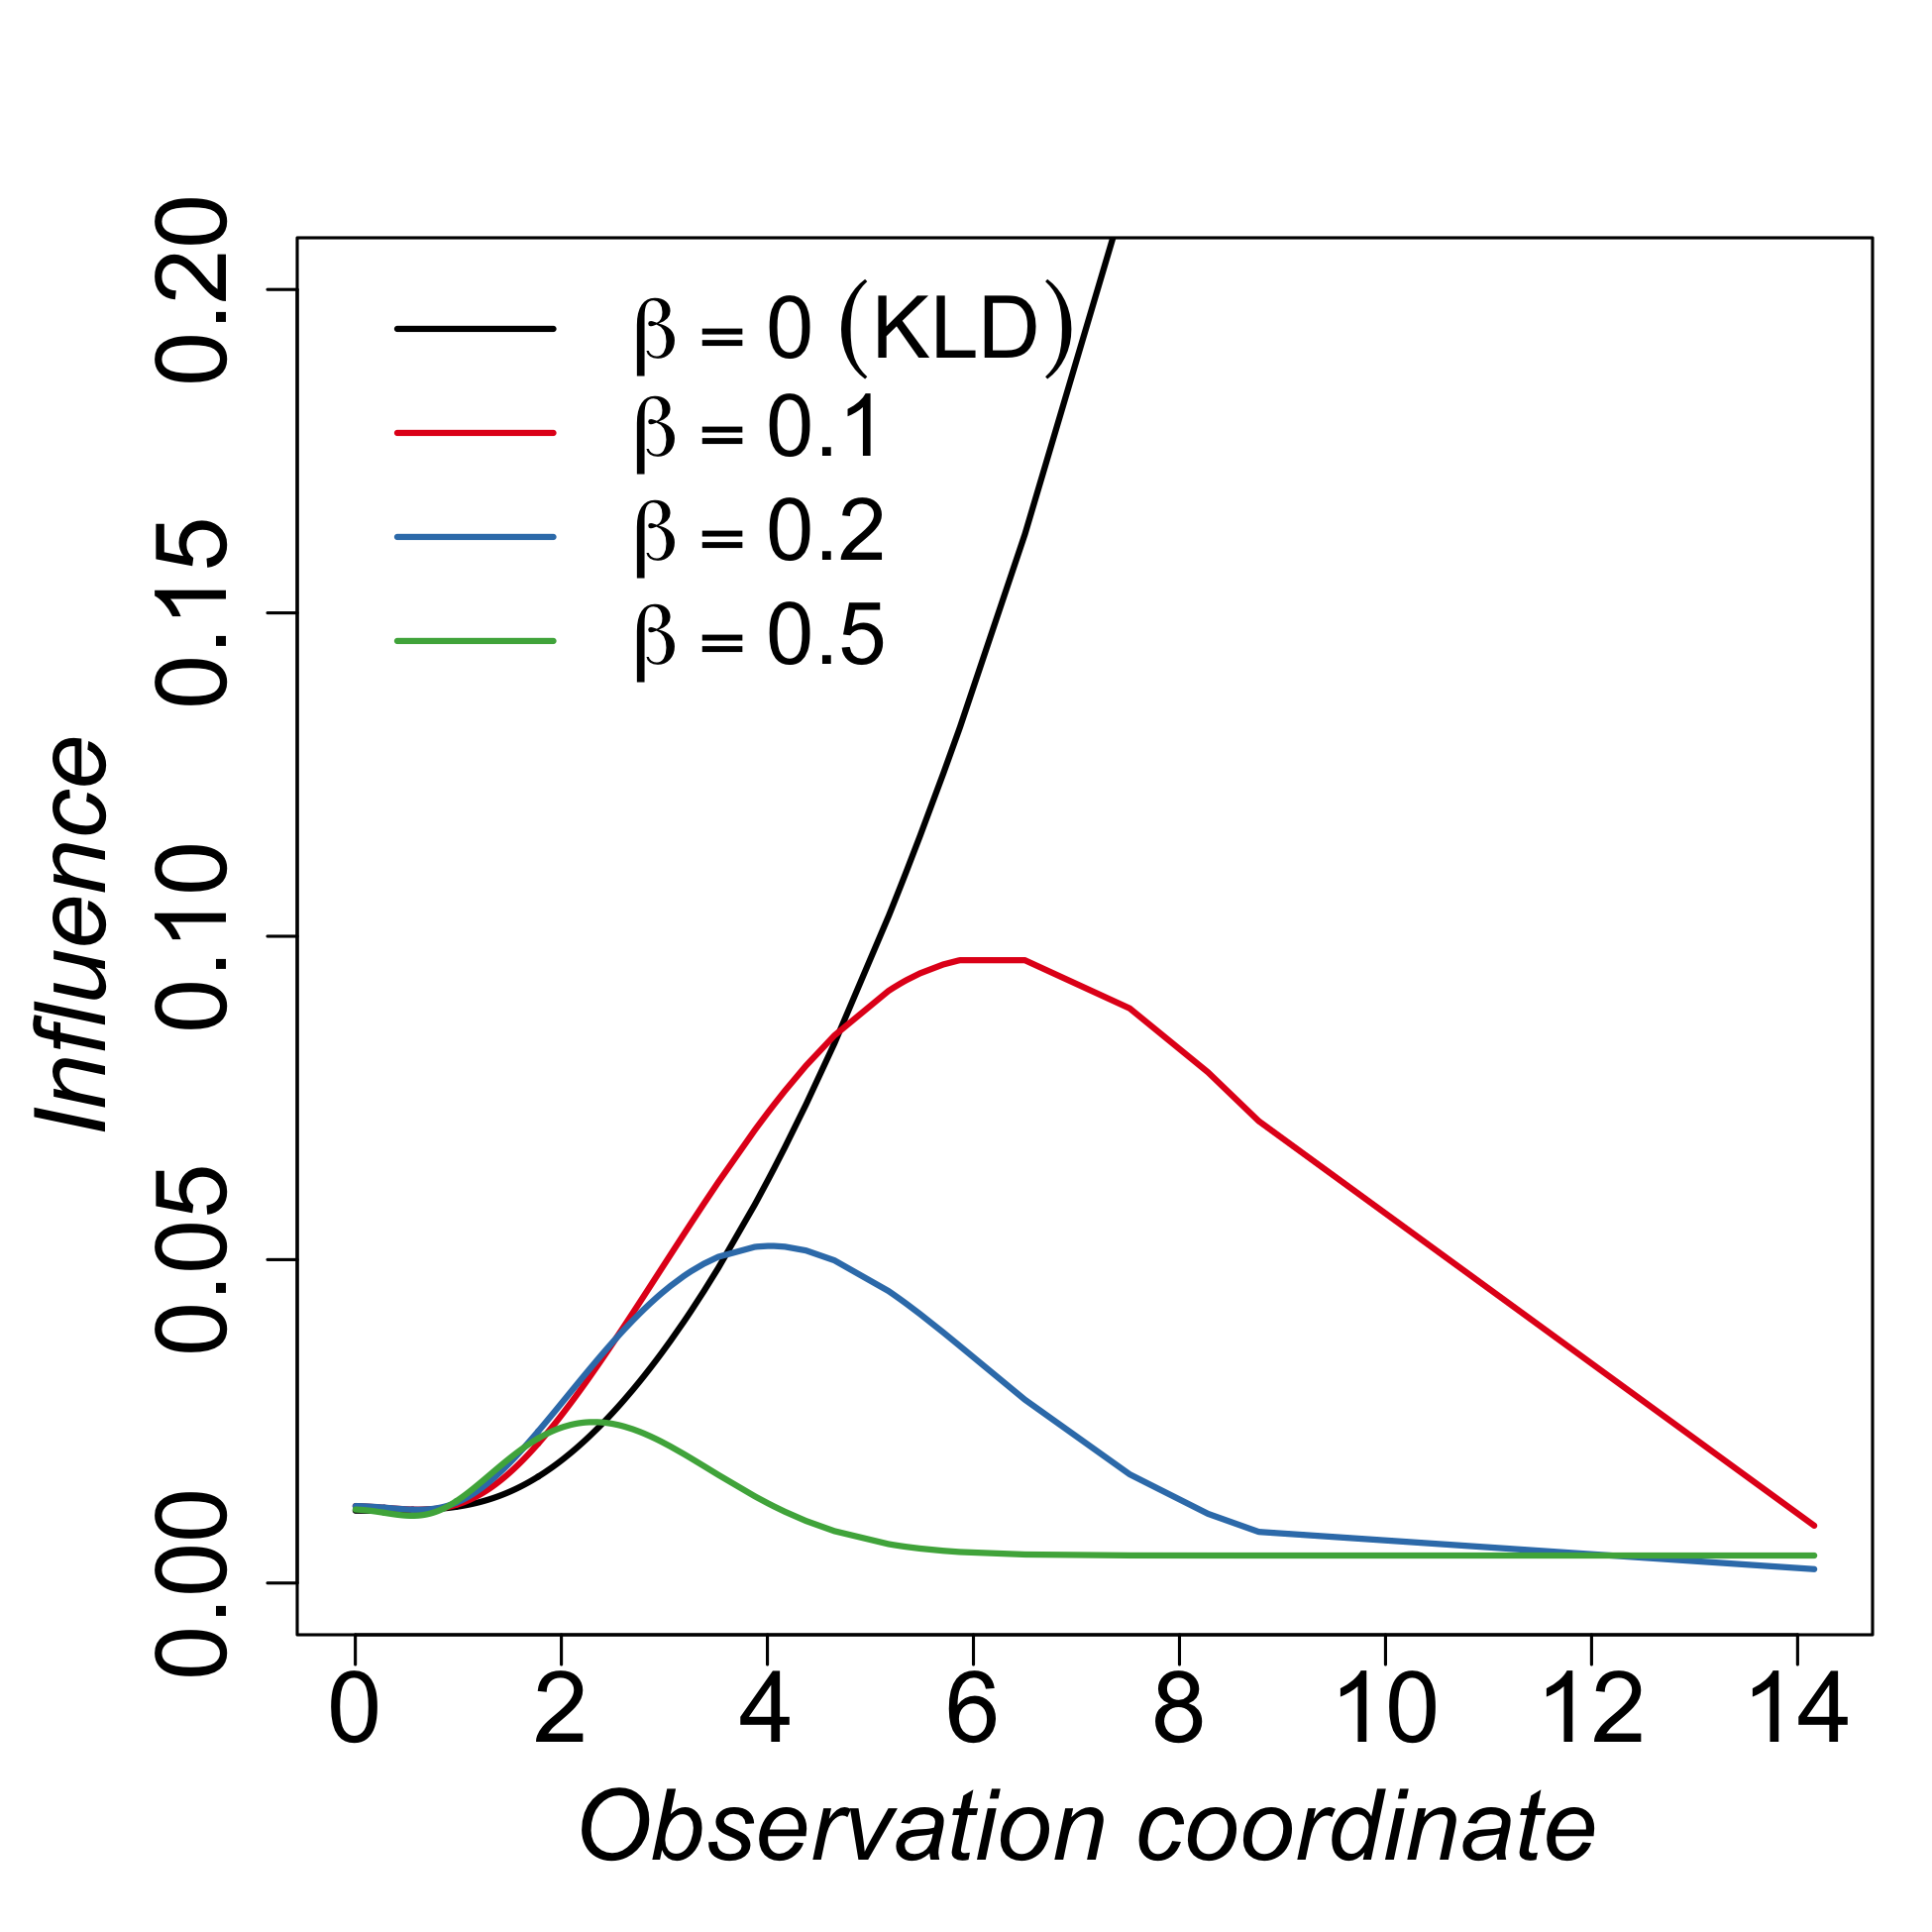
\includegraphics[width=.99\textwidth]{\PathChapter/figs/influence.png}
	\caption{\centering {}}
	\label{fig:influence}
	\end{subfigure}	
	\begin{subfigure}[t]{0.49\textwidth} 
	\centering
	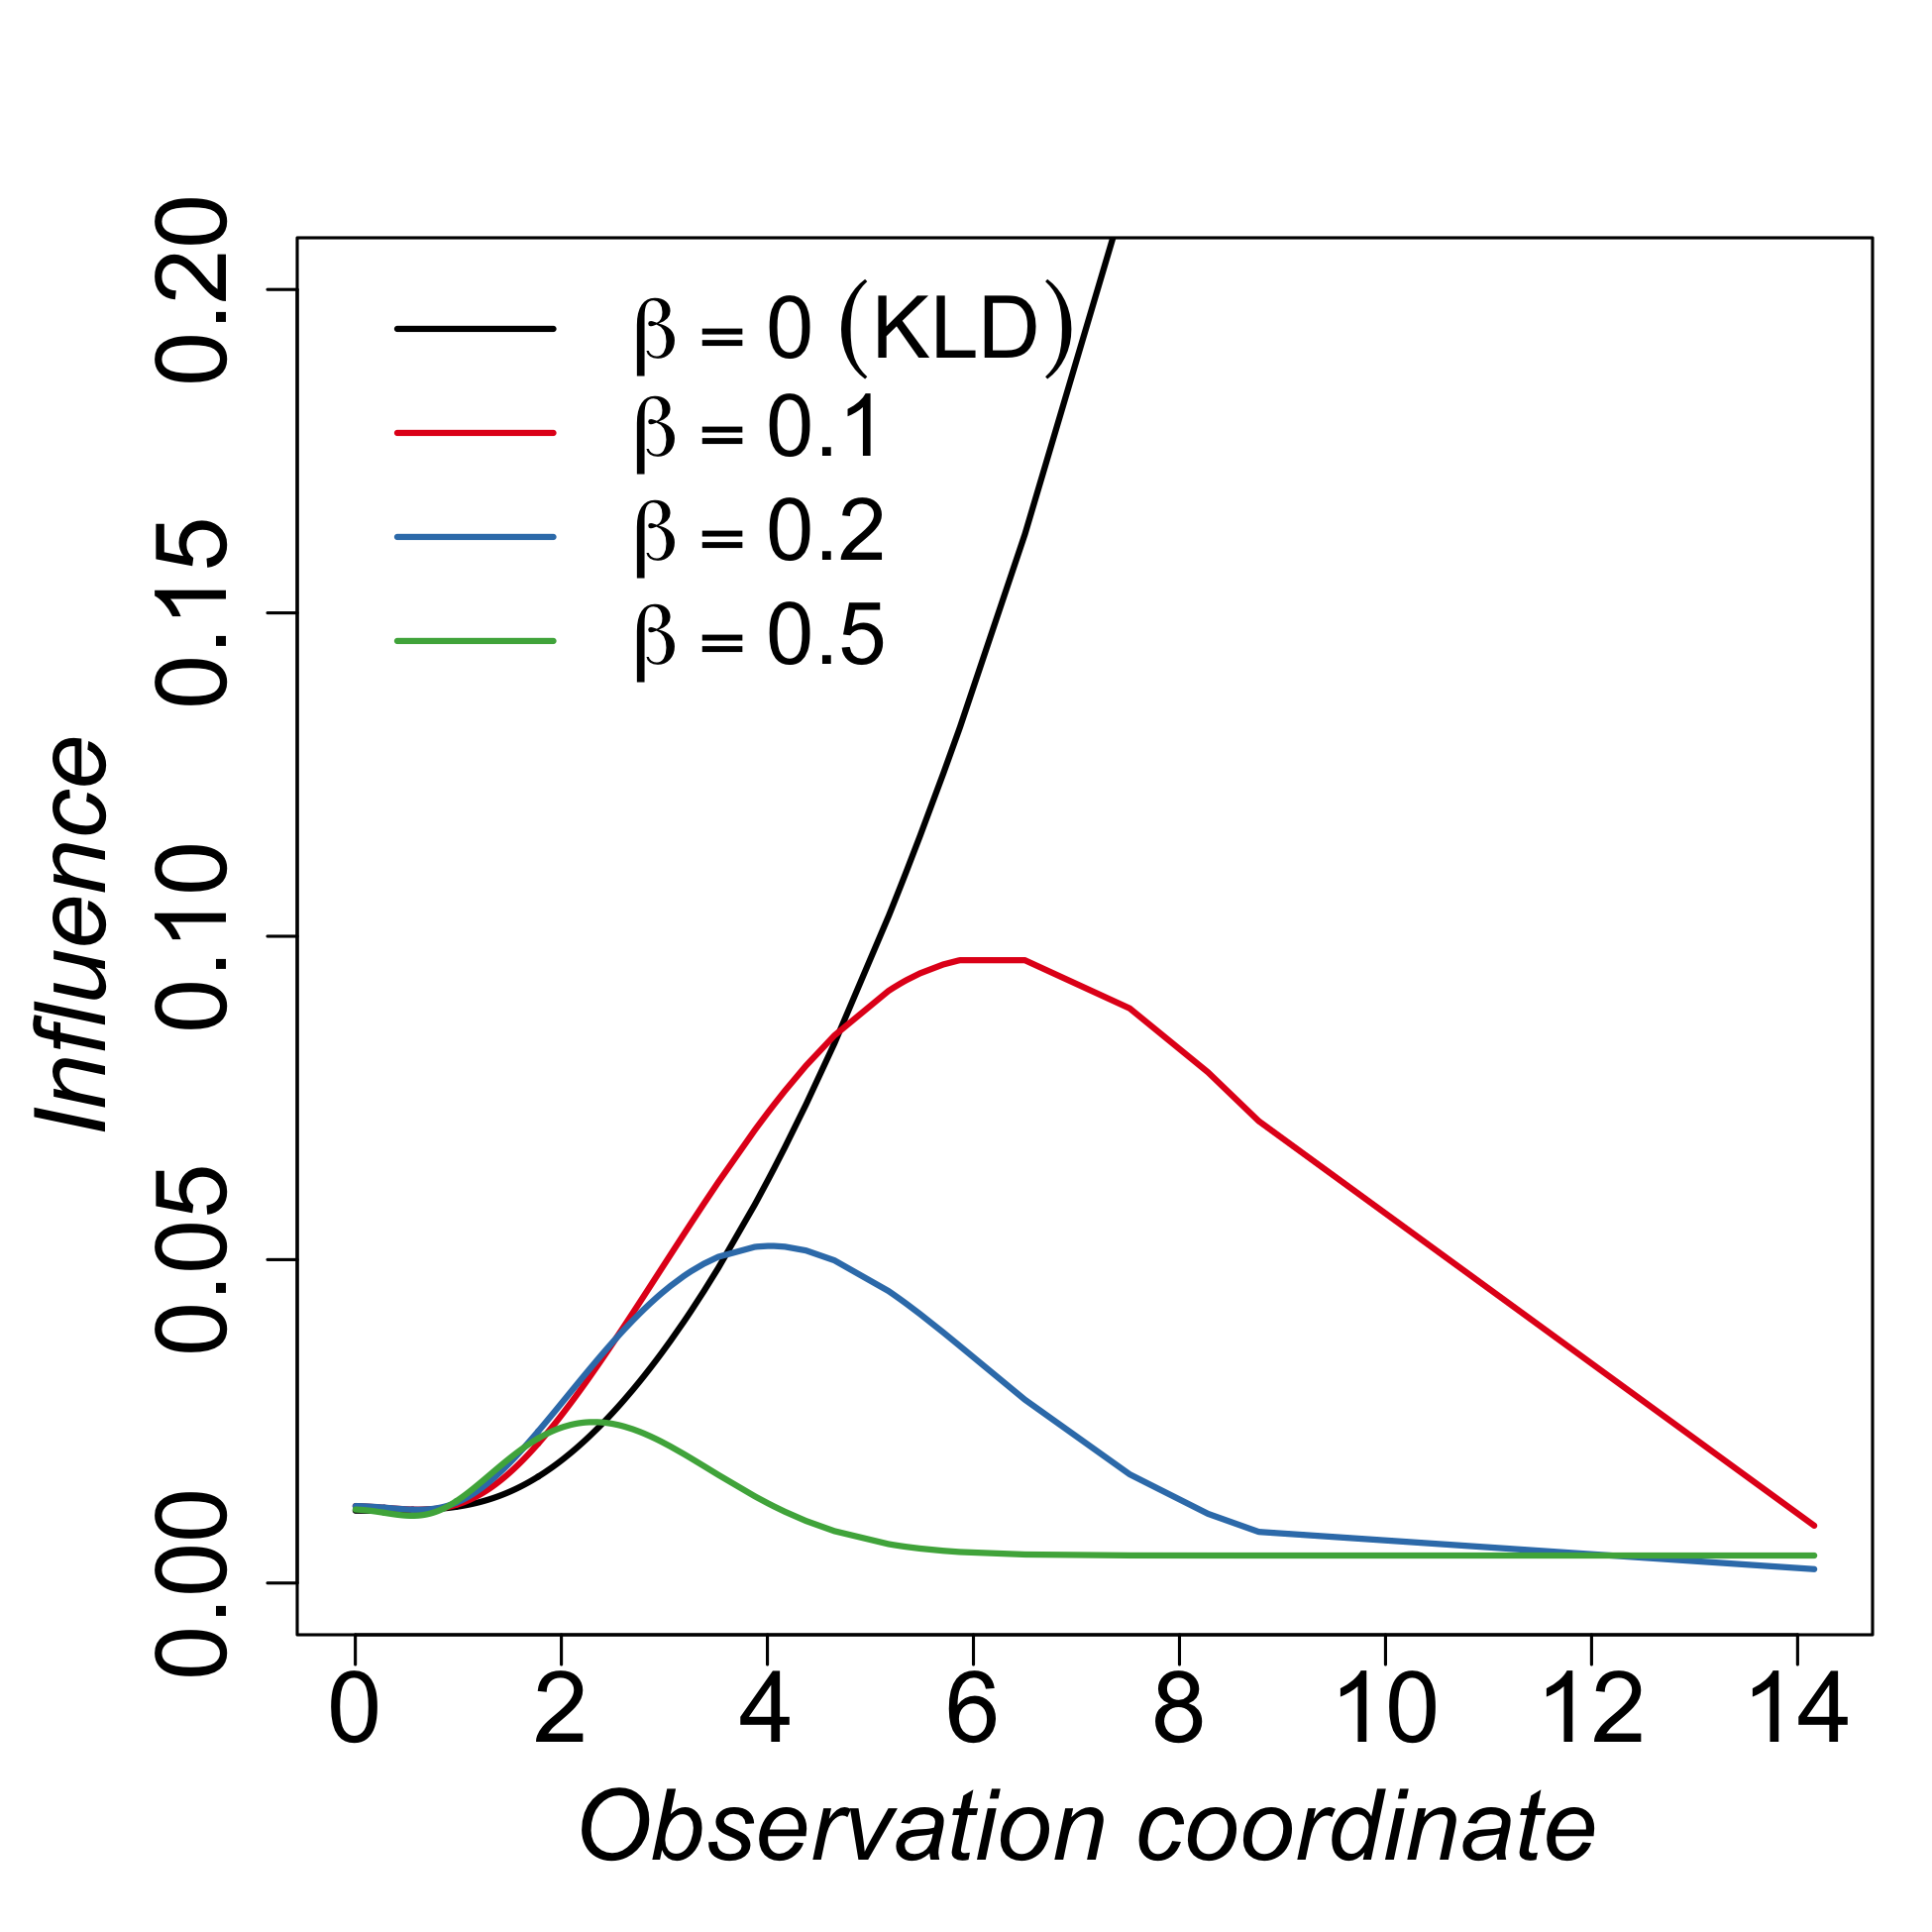
\includegraphics[width=.99\textwidth]{\PathChapter/figs/influence.png}
	\caption{\centering {}}
	\label{fig:influence-b}
	\end{subfigure}	
	\caption{Effects of altering the statistical divergence when conducting inference on datasets containing outliers. (\subref{fig:influence})~The influence of individual datapoints under the Kullback-Leibler and the $\beta$-divergence: the concavity of influence under the $\beta$-divergence illustrates the robustness of the inferred posterior to outliers.}
	\label{fig:robust-inference}
\end{figure*}

~\cref{fig:influence} demonstrates the \emph{influence} of individual observations with varying magnitude on the posterior for a Gaussian with unknown mean and variance. The influence is measured using the Fisher--Rao metric introduced in~\citep{kurtek15}. For this experiment, $10K$ observations were sampled from a Student $t(3)$ distribution, while observations with negative coordinates were omitted from the presented plot due to symmetry. We can notice that the KL divergence allows unbounded influence, indicating the brittleness of inference on the tails of the observed distribution. In contrast, moving away from the mean, individual datapoints' influence under the $\beta$-divergences is initially characterised by a regime of increase until reaching a maximum (which depends on the selected robustness hyperparameter), succeeded by attenuation down to zero at the tails of the data distribution. At the same time, this experiment makes clear that for decision problems relying on the tail information of the observations, KL might be the divergence of choice, as the power density divergence would downweight the importance of datapoints lying far from the mean.   


\section{Representing data}
\label{sec:b-representing-data}
Extracting a relevant feature representation is an important step in the context of statistical pattern recognition. For this purpose a feature map 
\[
\phi: \mcX \rightarrow \mcH,
\]
is sought which transforms the datapoints from the original data space $\{x_n\}_{n=1}^{N}$, $x_n \in \mcX$, into \emph{feature representations} in a Hilbert space $\{\phi(x_n)\}_{n=1}^{N}$, $\phi(x_n) \in \mcH$. Then the patterns of interest can be revealed via applications of inner products in the Hilbert space $\langle A, \phi(x) \rangle_{\mcH}$. There is an extensive literature on constructing data representations; for the purposes of this thesis, in the remainder of the section we focus on two of them: kernel methods and random projections.


\subsection{Kernels}
\label{subsec:b-kernels}

The main tool in kernel methods~\citep{scholkopf02} is the \emph{kernel function} defined below.
\begin{ndefn}[Kernel function] \label{def:bkernelfun}
	A symmetric function $k: \mcX \times \mcX \rightarrow \reals $ is a positive semidefinite \emph{kernel function}, or \emph{kernel}, if for all $N>1$, $x_1, \ldots, x_N \in \reals$, and $c_1, \ldots, c_N \in \reals$ 
	\[
	\sum_{i,j=1}^{N} c_ic_j k(x_i, x_j) \geq 0.
	\]
\end{ndefn}

Every kernel is associated with a feature map $\phi$ as follows.

\begin{ndefn}[Kernel representation] \label{def:bkernelrepr}
	 A function $k: \mcX \times \mcX \rightarrow \reals$ is a kernel iff there exists a Hilbert space $\mcH$ and a feature map $\phi: \mcX \rightarrow \mcH$ such that for all $x, x' \in \mcX$
	 \[
	 \label{eq:bkernelrep}
	 k(x,x') = \langle \phi(x), \phi(x') \rangle_\mcH.
	 \]
	 Feature map $\phi$ endows each datapoint $x \in \mcX$ with a kernel representation $\phi(x)$.
\end{ndefn}
A kernel representation might be lacking an explicit closed form, but can always be accessed via the inner product of~\cref{eq:bkernelrep}, which is the central object of interest in learning with kernels.

Examples of widely-used kernel functions include:
\begin{itemize}
	\item The (inhomogeneous) polynomial kernel $k(x,x') = \left(\langle x, x'\rangle + c\right)^d$, where $ {c \geq 0}, {d \in \nats}$.
	\item The Gaussian kernel $k(x,x') = \exp(-\gamma||x-x'||_{2}^2)$.
	\item Radial Basis Function~(RBF) kernels $k(x,x') = f(d(x,x'))$, where $d$ is a metric on $\mcX$ and $f$ is a function on $\reals^{+}$.
\end{itemize}

Kernel methods induce \emph{non-parametric} representations on the data, \ie~when given a set with $ N $ datapoints of dimension $d$, kernels effectively map each datapoint to an $N$-dimensional representation. %Although allowing representation power scaling with the number of datapoints, such methods often reach prohibitive computational cost.

\subsection{Finite-dimensional random projections}
\label{subsec:b-random-features}

Kernel methods appeal to large-scale learning due to their non-parametric nature: their representation power scales with the number of datapoints, hence they can learn complex, highly non-linear structure from the data; however, their time and memory cost scales adversely with the dataset size. Random features~\citep{rahimi08} remedy poor complexity scaling issues via utilising \emph{parametric finite-dimensional} data representations. We motivate this concept via an application arising in Hilbert coreset constructions~\citep{campbell19jmlr}.

Denote by $ f_n(\theta) \defined \sum_{n=1}^{N} \log\pi(x_n|\theta) $ the log-likelihood function of a dataset $x \defined {(x_n)}_{n=1}^{N}$, and by $ f(\theta,w) \defined \sum_{n=1}^{N} w_n\log\pi(x_n|\theta)$ the corresponding log-likelihood of a Hilbert coreset $(w_n, x_n)_{n=1}^{N}$ constructed on the data, where $(w_n)_{n=1}^{N}$ is a vector of sparse, non-negative weights---using the simplified notation $f(\theta)$ for the full data log-likelihood. The quality of posterior approximation that this coreset offers can be quantified using a $L^2$ norm on the log-likelihoods under a weighting distribution $\hpi$ that has the same support with the true posterior $\pi$ 
\[
||f(\theta, w) - f(\theta)||_{\hpi,2} \defined \EE_{\hpi} \left[ (f(\theta) - f(\theta, w))^2\right],
\]
and induced inner product
\[
\label{eq:binner-prod-hc}
\langle f_n(\theta), f_m(\theta) \rangle_{\hpi, 2} \defined \EE_{\hpi}\left[f_n(\theta), f_m(\theta)\right].
\]
The weighting distribution $\hpi$ can be selected from a set of cheap posterior approximations, for example using Laplace's method, or running a few rounds of an MCMC algorithm. In the general case, the norm of~\cref{eq:binner-prod-hc} is not available in closed form, hence a random projection can be used instead to approximate it according to the following steps:
\begin{enumerate}
	\item Sample $J$ values for $\theta$ from the weighting distribution $(\htheta_j)_{j=1}^{J} \distiid \hpi$.
	\item For $n=1 \ldots N$ compute a $J$-dimensional projection $ \hf_n(\theta) \defined \sqrt{\frac{1}{J}}[f_n(\htheta_1) \ldots f_n(\htheta_J)]$.
\end{enumerate}
In this way we get an unbiased finite-dimensional estimator of the inner products
\[
\langle f_n(\theta), f_m(\theta) \rangle_{\hpi, 2}  \approx \hf_n(\theta)^T \hf_m(\theta).
\]


\section{Differential privacy}
\label{sec:bdp}

Differential privacy~(DP)~\citep{dwork2006calibrating,dwork14} is a formal framework quantifying the privacy threat that exists in observing the output of a data analysis task carried out on a sensitive database, due to changing an individual entry of its input. The central model of DP considers a setting where the database is held by a trusted curator; and an untrusted analyst sends statistical queries to the curator and receives public responses via randomized algorithms, or \emph{mechanisms}: DP enforces a stability property on the output distribution of these mechanisms that limits the disclosure of information about any individual record within the database, offering strong indistinguishability guarantees regardless of the side information that the analyst might possess~(even when the analyst knows all other records of the database). 

DP definition requires a notion of \emph{neighboring} databases.
To define distance between two databases $x, x' \in \mcX$ of size $ N $ we use the Hamming distance
\[
D_{H}(x, x') \defined \#\{n=1,\ldots,N: x_n \neq x'_n \}.
\]
We call the databases adjacent, denoted $ x \approx x'$, iff $D_{H}(x, x')=1$.


\label{sec:b-differential-privacy}
\ndefn[Differential Privacy]{
	Fix $\veps \geq $, $\delta \geq 0$. A mechanism $ \mcM: \mcX \rightarrow \mcY$  is $(\veps, \delta)$-differentially private if for all adjacent datasets $ x \approx x'$ and each event $ A \subseteq \mcY$, 	$\;\Pr[\mcM(x) \in A] \leq e^\veps \Pr[\mcM(x') \in A] + \delta$.
	\label{def:b-dp-definition}
}

\cref{def:b-dp-definition} with $\delta=0$, known as \emph{pure DP}, requires that if we perturb a database by a single datapoint, the output of the algorithm should not differ much, with the privacy risk being controlled by the parameter $\veps$.
A weaker definition of DP allows that the guarantee of~\cref{def:b-dp-definition} gets broken with probability $\delta>0$. This corresponds to the notion of \emph{($\veps, \delta$)-approximate differential privacy}. The latter generally allows more tools for tighter privacy analysis over repeated access to the data, and will be the definition applied on our privacy-preserving summarization scheme in~\cref{chap:chap4}. In practice, $\veps \leq 0.1$ and $\delta \approx 1/N^{\omega(1)}$ are typically considered good values for the privacy parameters. 

The most common mechanisms that enable releasing numerical queries $f$ under DP rely on randomization via injecting additive noise. The amount of noise is calibrated to the \emph{global sensitivity} of the query, which is defined as 
\[
\Delta_p(f) := \underset{x \approx x'}{\max} ||f(x)-f(x')||_p.
\]
To achieve $(\veps, \delta)$-DP one can use the Gaussian Mechanism, which returns
\[
f(x)+Z, \quad Z \sim \mcN(0, \sigma^2 I), \quad \text{where } \sigma \geq \frac{\sqrt{2\log(1.25/\delta)}\Delta_2(f)}{\veps}.
\]

DP is equipped with a suite of properties that facilitate reasoning about privacy guarantees over complicated analysis tasks on a sensitive data collection in a modular fashion. In the remainder we review a fraction of them which are frequently encountered in machine learning settings.

A useful fact about DP algorithms is that a data analyst cannot weaken their privacy guarantees by doing any computation on their output that does not depend on the private input itself.

\bnprop[Robustness to Post-Processing~\citep{dwork14}]
	Let $ {\mcM: \mcX \rightarrow \mcY}$ be $(\veps, \delta)$-DP and $\psi:\mcY \rightarrow \mcY'$ be any function. Then $\psi \circ \mcM: \mcX \rightarrow \mcY'$ is $(\veps, \delta)$-DP.
	\label{prop:bdp-postprocessing}
\enprop

Moreover, running a mechanism on a random subset of the datapoints implies stronger privacy compared to running the mechanism on the full database.

\bnprop[Privacy Amplfication via Random Sampling~\citep{kasiviswanathan11,beimel13}]
Let $ \mcM: \mcX \rightarrow \mcY$ be $(\veps, \delta)$-DP with $\veps \leq 1$ and $\upsilon: \mcX \rightarrow \mcX$, a random sampler returning a random ratio $q$ of the datapoints. Then $\mcM \circ \upsilon: \mcX \rightarrow \mcY$ is $(O(q\veps), q\delta)$-DP.
\label{prop:bdp-sampling}
\enprop

DP composition theorems accumulate the total privacy cost over the application of a sequence of mechanisms. The moments accountant is a recently proposed technique, that allows computing tight bounds for $\veps$ and $\delta$, offering the following guarantees:

\bnprop[Moments Accountant~\citep{abadi16}]
Given $0<\veps<1$ and $0<\delta<1$, to ensure $(\veps, T\delta'+\delta)$-DP over the composition of $T$ mechanisms $\mcM_1,\ldots,\mcM_T$, it suffices that each $\mcM_i$ is $(\veps', \delta')$-DP, where $\veps'=\frac{\veps}{2\sqrt{2T\log(2/\delta)}}$ and $\delta'=\frac{\delta}{T}$. 
\label{prop:bmoments-accountant}
\enprop

The above tools are required for carrying out the privacy analysis of the \emph{subsampled Gaussian mechanism}~\citep{abadi16}, which will be used for privatising the variational inference scheme introduced in~\cref{chap:chap4}.



